\subsection{Mathematical Language, Sets, and Functions}


This subsection fixes the language used throughout Analysis: membership, containment, functions, images, preimages, and the basic proof patterns for unpacking definitions. Later sections should cite these labels rather than reintroducing elementary set and function calculus.

\begin{principle} \label{princ:analysis-language-as-structure} \hlt{Language Carries Structure}\\
Objects, hypotheses, conclusions, and quantifier order matter. For instance,
\begin{align}
\forall x\in X\ \exists y\in Y\ P(x,y), \qquad
\exists y\in Y\ \forall x\in X\ P(x,y) \nonumber
\end{align}
are different: in the first $y$ may depend on $x$; in the second one $y$ works for all $x$.
\end{principle}

\begin{principle} \label{princ:well-formed-statements-and-bound-variables} \hlt{Well-Formed Statements and Bound Variables}\\
A mathematical statement is well formed only after every symbol has a declared role and every expression has a defined meaning. A variable introduced by a quantifier, summation sign, integral, set-builder condition, or similar construction is \hlt{bound} inside that construction; changing its name does not change the statement as long as its scope is unchanged and no free variable is captured.
\end{principle}

\begin{principle} \label{princ:mathematical-induction} \hlt{Mathematical Induction}\\
Let $P_1,P_2,\ldots$ be statements indexed by positive integers. To prove $P_n$ for every $n\in\N$, it is enough to prove:
\begin{enumerate}[label=(\roman*)]
\setlength{\itemsep}{0pt}
\item \hlt{basis}: $P_1$ is true;
\item \hlt{induction step}: for every $n\in\N$, $P_n$ implies $P_{n+1}$.
\end{enumerate}
The induction step is an implication; it does not prove $P_{n+1}$ in isolation.\\
The basis starts the chain, and the implication carries truth from one statement to the next.
\end{principle}

\begin{figure}[H]
  \centering
  \begin{tikzpicture}[
  >=Stealth,
  every node/.style={font=\small},
  value/.style={rounded corners=2pt, draw=orange!70!black, fill=orange!10, minimum width=10mm, minimum height=7mm, inner xsep=4pt, line width=0.55pt},
  arrow/.style={->, line width=0.5pt, gray!62},
  rowlabel/.style={anchor=east, gray!68, font=\small},
  rowsub/.style={anchor=east, gray!58, font=\scriptsize}
]
  \path[use as bounding box] (-2.65,-1.85) rectangle (6.25,0.52);

  \node[rowlabel] at (-0.72,0.12) {induction};
  \node[rowsub] at (-0.72,-0.18) {base + step};
  \node[value] (p0) at (0,0) {$P(0)$};
  \node[value] (p1) at (1.55,0) {$P(1)$};
  \node[value] (p2) at (3.10,0) {$P(2)$};
  \node[value] (p3) at (4.65,0) {$P(3)$};
  \node at (5.85,0) {$\cdots$};

  \draw[arrow] (p0) -- (p1);
  \draw[arrow] (p1) -- (p2);
  \draw[arrow] (p2) -- (p3);
  \draw[arrow] (p3) -- (5.55,0);

  \node[rowlabel] at (-0.72,-1.28) {recursion};
  \node[rowsub] at (-0.72,-1.58) {initial + rule};
  \node[value] (a0) at (0,-1.40) {$a_0=c$};
  \node[value] (a1) at (1.55,-1.40) {$a_1$};
  \node[value] (a2) at (3.10,-1.40) {$a_2$};
  \node[value] (a3) at (4.65,-1.40) {$a_3$};
  \node at (5.85,-1.40) {$\cdots$};

  \draw[arrow] (a0) -- (a1);
  \draw[arrow] (a1) -- (a2);
  \draw[arrow] (a2) -- (a3);
  \draw[arrow] (a3) -- (5.55,-1.40);
\end{tikzpicture}

  \caption{Induction propagates truth, while recursion propagates values along the same index chain.}
  \label{fig:peano-recursion-induction-ladder}
\end{figure}

\begin{method} \label{meth:proof-grammar-and-negation} \hlt{Proof Grammar and Negation}\\
In theorem statements, put the hypotheses before the conclusion and keep quantifiers in the order meant.\\
In particular, switching $\forall$ and $\exists$ usually changes the statement; see Principle \ref{princ:analysis-language-as-structure}.\\
Before applying a rule, also check that the displayed expressions are well formed; an undefined expression makes the sentence ill formed, not merely false.\\
The word ``or'' is inclusive in mathematics, and the basic negation rules are
\begin{align}
\neg(a\land b)\Longleftrightarrow \neg a\lor\neg b, \qquad \neg(a\lor b)\Longleftrightarrow \neg a\land\neg b, \qquad \neg(a\Rightarrow b)&\Longleftrightarrow a\land\neg b \nonumber
\end{align}
Thus a proof by contradiction of $a\Rightarrow b$ assumes both $a$ and $\neg b$ and derives an impossibility.\\
\hlt{Key Insight}: Before proving or negating a statement, parse its quantifiers and logical connectives.
\end{method}

\begin{definition} \label{def:analysis-sets-and-operations} \hlt{Sets and Operations}\\
A \hlt{set} is a collection. Write $x\in E$, $x\notin E$, $\emptyset$, and $A\subseteq B$; $A=B$ iff $A\subseteq B$ and $B\subseteq A$. For $A,B\subseteq X$,
\begin{align}
A\cup B &\defeq \{x\in X:x\in A\text{ or }x\in B\}, \nonumber\\
A\cap B &\defeq \{x\in X:x\in A\text{ and }x\in B\}, \nonumber\\
A\setminus B &\defeq \{x\in X:x\in A\text{ and }x\notin B\}, \nonumber\\
A^c &\defeq X\setminus A. \nonumber
\end{align}
The \hlt{power set} is $\mathcal{P}(X)\defeq\{A:A\subseteq X\}$.
\end{definition}

\begin{remark} \label{rem:set-builder-notation} \hlt{Set-Builder Notation}\\
$\{x\in X:P(x)\}$ means all $x\in X$ satisfying $P(x)$.\\
For sets $(A_n)$, $\bigcup_nA_n$ means membership in some $A_n$; $\bigcap_nA_n$, membership in every $A_n$.\\
\hlt{Key Insight}: Expand membership conditions.
\end{remark}

\begin{definition} \label{def:indexed-families-unions-intersections} \hlt{Indexed Families of Sets}\\
An \hlt{indexed family} $\{A_i\}_{i\in I}$ is one set $A_i\subseteq X$ for each index $i\in I$. Define
\begin{align}
\bigcup_{i\in I}A_i&\defeq\{x\in X:x\in A_i\text{ for some }i\in I\}, \nonumber\\
\bigcap_{i\in I}A_i&\defeq\{x\in X:x\in A_i\text{ for every }i\in I\}. \nonumber
\end{align}
\hlt{Key Insight}: Union means ``some index''; intersection means ``every index''.
\end{definition}

\begin{method} \label{meth:proof-by-containment} \hlt{Proof by Two Containments}\\
To prove $A=B$, prove both inclusions.
\begin{enumerate}[label=(\roman*)]
\setlength{\itemsep}{0pt}
\item To prove $A\subseteq B$, let $x\in A$ be arbitrary and use the definitions and hypotheses to show $x\in B$.
\item To prove $B\subseteq A$, let $x\in B$ be arbitrary and use the definitions and hypotheses to show $x\in A$.
\item Once both containments are proved, conclude $A=B$ by extensionality of sets.
\end{enumerate}
If both sides are described by membership conditions, this is a chain, $x\in A \Longleftrightarrow \cdots \Longleftrightarrow x\in B$.
\end{method}

\begin{proposition} \label{prop:analysis-set-algebra} \hlt{Basic Set Algebra}\\
Let $A,B,C\subseteq X$. Then
\begin{enumerate}[label=(\roman*)]
\setlength{\itemsep}{0pt}
\item $A\cap(B\cup C)=(A\cap B)\cup(A\cap C)$;
\item $A\cup(B\cap C)=(A\cup B)\cap(A\cup C)$;
\item $(A\cup B)^c=A^c\cap B^c$;
\item $(A\cap B)^c=A^c\cup B^c$.
\end{enumerate}
\begin{proof}
It suffices to prove (i) and (iii); the others are similar. Let $x\in X$. Then
\begin{enumerate}[label=(\roman*)]
\setlength{\itemsep}{0pt}
\item[(i)] $x\in A\cap(B\cup C) \Longleftrightarrow x\in A \text{ and } (x\in B \text{ or } x\in C) \Longleftrightarrow (x\in A\cap B) \text{ or } (x\in A\cap C) \Longleftrightarrow x\in (A\cap B)\cup(A\cap C)$
\item[(iii)] $x\in (A\cup B)^c \Longleftrightarrow x\notin A\cup B \Longleftrightarrow x\notin A \text{ and } x\notin B \Longleftrightarrow x\in A^c\cap B^c$
\end{enumerate}
\hlt{Structural Commentary}: Set algebra is membership logic.\\
\hlt{Key Insight}: Translate sets into conditions on $x$.
\end{proof}
\end{proposition}

\begin{figure}[H]
    \centering
    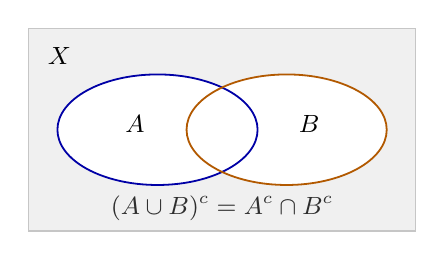
\begin{tikzpicture}[
  x=0.82cm,
  y=0.78cm,
  every node/.style={font=\small},
  ambient/.style={draw=gray!45, fill=gray!12, line width=0.5pt},
  setA/.style={draw=blue!65!black, line width=0.65pt},
  setB/.style={draw=orange!70!black, line width=0.65pt}
]
  \draw[ambient] (-3,-1.65) rectangle (3,1.65);
  \fill[white] (-1.0,0) ellipse (1.55 and 0.9);
  \fill[white] (1.0,0) ellipse (1.55 and 0.9);
  \draw[setA] (-1.0,0) ellipse (1.55 and 0.9);
  \draw[setB] (1.0,0) ellipse (1.55 and 0.9);

  \node at (-1.35,0.1) {$A$};
  \node at (1.35,0.1) {$B$};
  \node[anchor=north west] at (-2.85,1.5) {$X$};
  \node[gray!35!black] at (0,-1.28) {$(A\cup B)^c=A^c\cap B^c$};
\end{tikzpicture}

    \caption{De Morgan's law says that being outside a union is the same as being outside each set.}
    \label{fig:de-morgan-complement-union}
\end{figure}

\begin{definition} \label{def:cartesian-product} \hlt{Cartesian Product}\\
For sets $X$ and $Y$, the \hlt{Cartesian product} is $X\times Y\defeq\{(x,y):x\in X,\ y\in Y\}$.\\
The order matters: the first coordinate comes from $X$, and the second comes from $Y$.
\end{definition}

\begin{figure}[H]
    \centering
    \begin{tikzpicture}[
  >=Stealth,
  every node/.style={font=\small},
  axis/.style={->, gray!65, line width=0.45pt},
  interval/.style={line width=1.2pt},
  product/.style={draw=blue!60!black, fill=blue!8, line width=0.55pt},
  guide/.style={gray!55, dashed, line width=0.4pt},
  point/.style={circle, fill=black, inner sep=1.2pt}
]
  \draw[axis] (-0.25,0) -- (5.3,0);
  \draw[axis] (0,-0.25) -- (0,3.5);

  \coordinate (A0) at (1.15,0);
  \coordinate (A1) at (4.55,0);
  \coordinate (B0) at (0,0.8);
  \coordinate (B1) at (0,2.85);

  \draw[product] (1.15,0.8) rectangle (4.55,2.85);
  \draw[interval, blue!60!black] (A0) -- (A1);
  \draw[interval, orange!75!black] (B0) -- (B1);

  \node[below=5pt, blue!60!black] at (4.25,0) {$A$};
  \node[left=5pt, orange!75!black] at (0,2.75) {$B$};
  \node[blue!55!black, anchor=south east] at (4.35,0.92) {$A\times B$};

  \coordinate (P) at (2.75,2.05);
  \draw[guide] (2.75,0) -- (P);
  \draw[guide] (0,2.05) -- (P);
  \node[point] at (P) {};
  \node[below=1pt] at (2.75,0) {$a$};
  \node[left=2pt] at (0,2.05) {$b$};
  \node[above right=2pt] at (P) {$(a,b)$};
\end{tikzpicture}

    \caption{$A\times B$: first coordinate in $A$, second in $B$.}
    \label{fig:cartesian-product-rectangle}
\end{figure}

\begin{definition} \label{def:relations-and-equivalence} \hlt{Relations and Equivalence}\\
A \hlt{relation} from $X$ to $Y$ is a subset $R\subseteq X\times Y$. If $(x,y)\in R$, one often writes $xRy$.\\
A relation $\sim$ on $X$ is an \hlt{equivalence relation} if, for all $x,y,z\in X$,
\begin{enumerate}[label=\roman*.]
\setlength{\itemsep}{0pt}
\item $x\sim x$;
\item $x\sim y$ implies $y\sim x$;
\item $x\sim y$ and $y\sim z$ imply $x\sim z$.
\end{enumerate}
The equivalence class of $x$ is $[x]\defeq\{y\in X:y\sim x\}$.
\end{definition}

\begin{proposition} \label{prop:equivalence-relations-partitions} \hlt{Equivalence Classes Partition the Set}\\
Let $\sim$ be an equivalence relation on $X$. Then the equivalence classes form a partition of $X$.
\begin{proof}
Every $x\in X$ lies in $[x]$ since $x\sim x$. If $[x]\cap[y]\neq\emptyset$, choose $z$ in the intersection.\\
Then $x\sim z\sim y$, so $u\in[x]$ implies $u\sim y$ and $u\in[y]$. Hence $[x]\subseteq[y]$, and symmetry gives equality.\\
\hlt{Structural Commentary}: Equivalence means partition.\\
\hlt{Key Insight}: Touching classes coincide.
\end{proof}
\end{proposition}

\begin{definition} \label{def:functions-images-preimages} \hlt{Functions, Images, and Preimages}\\
A \hlt{function} $f:X\to Y$ assigns to each $x\in X$ a unique element $f(x)\in Y$. The set $X$ is the domain and $Y$ is the codomain. The \hlt{range} of $f$ is $\operatorname{range}(f)\defeq f(X)\defeq\{f(x):x\in X\}$.\\
If $A\subseteq X$, the \hlt{image} of $A$ under $f$ is $f(A)\defeq\{f(x):x\in A\}$.\\
If $B\subseteq Y$, the \hlt{preimage} of $B$ under $f$ is $f^{-1}(B)\defeq\{x\in X:f(x)\in B\}$.\\
This does not require $f$ to have an inverse function.\\
If $A\subseteq X$, the \hlt{restriction} of $f$ to $A$ is denoted $f|_A:A\to Y$.\\
If $g:Y\to Z$, the \hlt{composition} $g\circ f:X\to Z$ is defined by $(g\circ f)(x)=g(f(x))$.\\
The \hlt{identity function} on $X$ is denoted $\operatorname{id}_X$.
\end{definition}

  \begin{figure}[H]
  \centering
  \begin{tikzpicture}[
  x=0.78cm,
  y=0.78cm,
  >=Stealth,
  every node/.style={font=\small},
  ambient/.style={draw=gray!35, line width=0.45pt},
  setregion/.style={draw=blue!65!black, fill=blue!8, line width=0.55pt},
  preimage/.style={draw=orange!75!black, fill=orange!12, line width=0.55pt},
  targetset/.style={draw=orange!75!black, fill=orange!10, line width=0.55pt},
  image/.style={draw=blue!65!black, fill=blue!14, line width=0.55pt},
  maparrow/.style={->, gray!58, line width=0.42pt},
  point/.style={circle, fill=gray!75, inner sep=1.25pt}
]
  \draw[ambient, fill=white] (0,0) rectangle (4.25,3.4);
  \draw[ambient, fill=gray!12] (5.65,0) rectangle (9.9,3.4);

  \node[anchor=north west] at (0.25,3.25) {$X$};
  \node[anchor=north west] at (5.9,3.25) {$Y$};

  \draw[preimage]
    plot[smooth cycle, tension=0.7] coordinates {
      (0.86,0.78)
      (0.76,1.52)
      (1.16,2.32)
      (2.03,2.72)
      (3.04,2.42)
      (3.48,1.55)
      (3.05,0.75)
      (1.86,0.48)
    };
  \node[orange!55!black] at (2.08,2.43) {$f^{-1}(B)$};

  \draw[setregion]
    plot[smooth cycle, tension=0.75] coordinates {
      (1.28,1.02)
      (1.27,1.58)
      (1.62,2.02)
      (2.25,2.08)
      (2.78,1.74)
      (2.72,1.10)
      (2.05,0.82)
    };
  \node[blue!60!black] at (2.02,1.47) {$A$};

  \draw[targetset]
    plot[smooth cycle, tension=0.75] coordinates {
      (6.38,0.72)
      (6.16,1.50)
      (6.55,2.45)
      (7.55,2.88)
      (8.72,2.55)
      (9.18,1.62)
      (8.75,0.72)
      (7.48,0.42)
    };
  \node[orange!55!black] at (8.55,2.28) {$B$};

  \draw[image]
    plot[smooth cycle, tension=0.75] coordinates {
      (6.84,1.08)
      (6.95,1.72)
      (7.45,2.06)
      (8.05,1.92)
      (8.28,1.32)
      (7.82,0.92)
      (7.20,0.88)
    };
  \node[blue!60!black] at (7.55,1.48) {$f(A)$};

  \node[point] (x1) at (1.70,1.30) {};
  \node[point] (x2) at (2.34,1.83) {};
  \node[point] (x3) at (3.04,1.95) {};
  \node[point] (x4) at (0.72,0.34) {};

  \node[point] (y1) at (7.23,1.12) {};
  \node[point] (y2) at (7.94,1.76) {};
  \node[point] (y3) at (8.56,1.98) {};
  \node[point] (y4) at (9.28,0.36) {};

  \draw[maparrow] (x1) .. controls (3.25,1.08) and (5.70,1.02) .. (y1);
  \draw[maparrow] (x2) .. controls (3.75,1.68) and (5.88,1.64) .. (y2);
  \draw[maparrow] (x3) .. controls (4.12,2.42) and (6.60,2.46) .. (y3);
  \draw[maparrow] (x4) .. controls (3.15,0.18) and (6.75,0.12) .. (y4);

  \node[gray!65] at (5.02,2.05) {$f$};
  \draw[->, gray!55, line width=0.55pt] (4.38,1.45) -- (5.48,1.45);
\end{tikzpicture}

  \caption{Image--preimage containment: $f(A)\subseteq B \Longleftrightarrow A\subseteq f^{-1}(B)$.}
  \label{fig:function-image-preimage}
\end{figure}

\begin{proposition} \label{prop:image-preimage-calculus} \hlt{Image and Preimage Calculus}\\
Let $f:X\to Y$, let $\{A_i\}_{i\in I}$ be a nonempty family of subsets of $X$, and let $\{B_i\}_{i\in I}$ be a nonempty family of subsets of $Y$. Then
\begin{enumerate}[label=(\roman*)]
\setlength{\itemsep}{0pt}
\item $f\left(\bigcup_{i\in I}A_i\right)=\bigcup_{i\in I}f(A_i)$;
\item $f\left(\bigcap_{i\in I}A_i\right)\subseteq\bigcap_{i\in I}f(A_i)$;
\item $f^{-1}\left(\bigcup_{i\in I}B_i\right)=\bigcup_{i\in I}f^{-1}(B_i)$;
\item $f^{-1}\left(\bigcap_{i\in I}B_i\right)=\bigcap_{i\in I}f^{-1}(B_i)$;
\item $f^{-1}(Y\setminus B)=X\setminus f^{-1}(B)$ for every $B\subseteq Y$;
\item $f(f^{-1}(B))=B\cap\operatorname{range}(f)$ for every $B\subseteq Y$.
\end{enumerate}
\begin{proof}
\begin{enumerate}[label=(\roman*)]
\setlength{\itemsep}{0pt}
\item $y\in f(\bigcup_i A_i)$ iff $y=f(x)$ for some $x\in A_i$ and some $i$, iff $y\in\bigcup_i f(A_i)$.
\item If $y=f(x)$ with $x\in\bigcap_i A_i$, then $y\in f(A_i)$ for every $i$.
\item $x\in f^{-1}(\bigcup_i B_i)$ iff $f(x)\in B_i$ for some $i$, iff $x\in\bigcup_i f^{-1}(B_i)$.
\item $x\in f^{-1}(\bigcap_i B_i)$ iff $f(x)\in B_i$ for every $i$, iff $x\in\bigcap_i f^{-1}(B_i)$.
\item For $x\in X$, $x\in f^{-1}(Y\setminus B) \Longleftrightarrow f(x)\notin B \Longleftrightarrow x\notin f^{-1}(B) \Longleftrightarrow x\in X\setminus f^{-1}(B)$
\item $y\in f(f^{-1}(B))$ iff $y=f(x)$ for some $x$ with $f(x)\in B$, iff $y\in B\cap\operatorname{range}(f)$.
\end{enumerate}
\hlt{Structural Commentary}: Preimages are Boolean-exact; images need not be.\\
\hlt{Key Insight}: Pull back conditions through $f$.
\end{proof}
\end{proposition}

\begin{definition} \label{def:injective-surjective-bijective} \hlt{Injective, Surjective, and Bijective Maps}\\
Let $f:X\to Y$.
\begin{enumerate}[label=\roman*.]
\setlength{\itemsep}{0pt}
\item $f$ is \hlt{injective} if $f(x_1)=f(x_2)$ implies $x_1=x_2$.
\item $f$ is \hlt{surjective} if $\operatorname{range}(f)=Y$.
\item $f$ is \hlt{bijective} if it is both injective and surjective.
\end{enumerate}
\end{definition}

\begin{figure}[H]
  \centering
  \begin{tikzpicture}[
  scale=0.80,
  >=Stealth,
  every node/.style={font=\scriptsize},
  set/.style={draw=gray!65, fill=gray!10, line width=0.45pt},
  point/.style={circle, fill=black, inner sep=1.05pt},
  missed/.style={circle, fill=white, draw=black, line width=0.45pt, inner sep=1.05pt},
  map/.style={->, gray!70, line width=0.48pt}
]
  \foreach \xshift in {0,4.2,8.4} {
    \begin{scope}[xshift=\xshift cm]
      \draw[set] (0,0) ellipse (0.6 and 1.15);
      \draw[set] (2.9,0) ellipse (0.6 and 1.15);
      \node at (0,-1.42) {$X$};
      \node at (2.9,-1.42) {$Y$};
    \end{scope}
  }

  \begin{scope}
    \coordinate (a1) at (0,0.72);
    \coordinate (a2) at (0,0.18);
    \coordinate (a3) at (0,-0.36);
    \coordinate (a4) at (0,-0.86);
    \coordinate (b1) at (2.9,0.58);
    \coordinate (b2) at (2.9,0.00);
    \coordinate (b3) at (2.9,-0.62);
    \foreach \p in {a1,a2,a3,a4,b1,b2,b3} \node[point] at (\p) {};
    \draw[map] (a1) -- (b1);
    \draw[map] (a2) -- (b2);
    \draw[map] (a3) -- (b2);
    \draw[map] (a4) -- (b3);
  \end{scope}

  \begin{scope}[xshift=4.2cm]
    \coordinate (a1) at (0,0.68);
    \coordinate (a2) at (0,0.02);
    \coordinate (a3) at (0,-0.68);
    \coordinate (b1) at (2.9,0.78);
    \coordinate (b2) at (2.9,0.24);
    \coordinate (b3) at (2.9,-0.28);
    \coordinate (b4) at (2.9,-0.82);
    \foreach \p in {a1,a2,a3,b1,b2,b3} \node[point] at (\p) {};
    \node[missed] at (b4) {};
    \draw[map] (a1) -- (b1);
    \draw[map] (a2) -- (b2);
    \draw[map] (a3) -- (b3);
  \end{scope}

  \begin{scope}[xshift=8.4cm]
    \coordinate (a1) at (0,0.62);
    \coordinate (a2) at (0,0.00);
    \coordinate (a3) at (0,-0.62);
    \coordinate (b1) at (2.9,0.62);
    \coordinate (b2) at (2.9,0.00);
    \coordinate (b3) at (2.9,-0.62);
    \foreach \p in {a1,a2,a3,b1,b2,b3} \node[point] at (\p) {};
    \draw[map] (a1) -- (b1);
    \draw[map] (a2) -- (b2);
    \draw[map] (a3) -- (b3);
  \end{scope}
\end{tikzpicture}

  \caption{Surjective: covers codomain; injective: no collisions; bijective: both.}
  \label{fig:injective-surjective-bijective-maps}
\end{figure}

\begin{theorem} \label{thm:bijective-iff-invertible-function} \hlt{Bijective Means Invertible}\\
A function $f:X\to Y$ is bijective iff there exists a function $g:Y\to X$ s.t. $g\circ f=\operatorname{id}_X$, $f\circ g=\operatorname{id}_Y$.\\
When such a function exists, it is unique and is denoted $f^{-1}:Y\to X$.
\begin{proof}
\begin{enumerate}[label=\roman*.]
\setlength{\itemsep}{0pt}
\item[$(\Rightarrow)$] If $f$ is bijective, define $g(y)$ as the unique $x$ with $f(x)=y$. Then $g\circ f=\operatorname{id}_X$ and $f\circ g=\operatorname{id}_Y$.
\item[$(\Leftarrow)$] If such a $g$ exists, applying $g$ to $f(x_1)=f(x_2)$ gives $x_1=x_2$, and $y=f(g(y))$ gives surjectivity.
\end{enumerate}
If $g$ and $h$ are two-sided inverses, then $g(y)=g(f(h(y)))=h(y)$, so the inverse is unique.\\
\hlt{Structural Commentary}: A true inverse undoes $f$ on both sides.\\
\hlt{Key Insight}: Bijective means exactly one preimage per output.
\end{proof}
\end{theorem}

\begin{example} \label{ex:square-map-image-preimage} \hlt{Image and Preimage for the Square Map}\\
Let $f:\R\to\R$ be given by $f(x)=x^2$. Then $f([-2,1])=[0,4]$, $f^{-1}([1,4])=[-2,-1]\cup[1,2]$. The map is not injective because $f(1)=f(-1)$, and it is not surjective as a map $\R\to\R$ because no real number maps to $-1$.
\end{example}
